\subsubsection{فعالیت بالا آوردن سر}

فعالیت بالا آوردن سر یکی از فعالیت‌هایی است که می‌تواند اطلاعات مهمی درباره قدرت عضلات گردن، کنترل تنه و توانایی انجام حرکات ضدجاذبه فراهم کند. در افراد مبتلا به ضعف عضلانی، اجرای این فعالیت ممکن است با کاهش دامنه حرکت، افزایش زمان اجرا، ناتوانی در حفظ وضعیت سر یا استفاده از الگوهای جبرانی در تنه و اندام‌ها همراه باشد. بنابراین، بررسی این فعالیت می‌تواند اطلاعات مفیدی درباره تفاوت میان سطوح عملکردی شبیه‌سازی‌شده فراهم کند و دامنه ارزیابی سامانه پیشنهادی را کامل‌تر سازد.

\paragraph{گزارش کلی فعالیت}

در فعالیت بالا آوردن سر، حرکت اصلی شامل جداکردن سر از سطح اتکا و حرکت آن در خلاف جهت نیروی جاذبه است. به همین دلیل، انتظار می‌رود حسگر نصب‌شده روی پیشانی نقش اصلی را در ثبت تغییرات حرکتی داشته باشد. تغییر زاویه سر، سرعت اجرای حرکت، دامنه جابه‌جایی و میزان نوسان هنگام بالا آوردن یا پایین آوردن سر می‌توانند در سیگنال‌های این حسگر مشاهده شوند.

نمونه سیگنال در
\autoref{fig:Rise_Head_normal_signal_sample}
نشان می‌دهد، با وجود تمرکز اصلی حرکت بر ناحیه سر و گردن، حسگرهای نصب‌شده روی دست‌ها نیز می‌توانند اطلاعاتی درباره حرکات جبرانی بدن فراهم کنند. برای مثال، حرکت دادن دست‌ها، ایجاد فشار روی سطح اتکا یا تغییر وضعیت اندام‌های تحتانی ممکن است به فرد در اجرای حرکت کمک کند.

\begin{figure}[H]
	\centering
	
\includegraphics[width=0.80\linewidth]{Images/Generated/TaskResults/Rise_Head/Normal/signal_sample.png}
	\caption{نمونه سیگنال‌های ثبت‌شده در فعالیت بالا آوردن سر}
	\label{fig:Rise_Head_normal_signal_sample}
\end{figure}

بعد از بررسی نمونه سیگنال، تمامی مراحل مانند فعالیت ایستادن صورت گرفت و تنها تفاوت در بررسی حالت جداسازی فعالیت بود که نتیجه آن در 
\autoref{fig:riseheadaccuracybaselinevsdetected}
آمده‌ است. این حالت تقریبا همان دقت حالت بدون جداسازی داشت بنابراین ادامه روند با همان داده‌های معمولی انجام شد.

\begin{figure}[H]
	\centering
	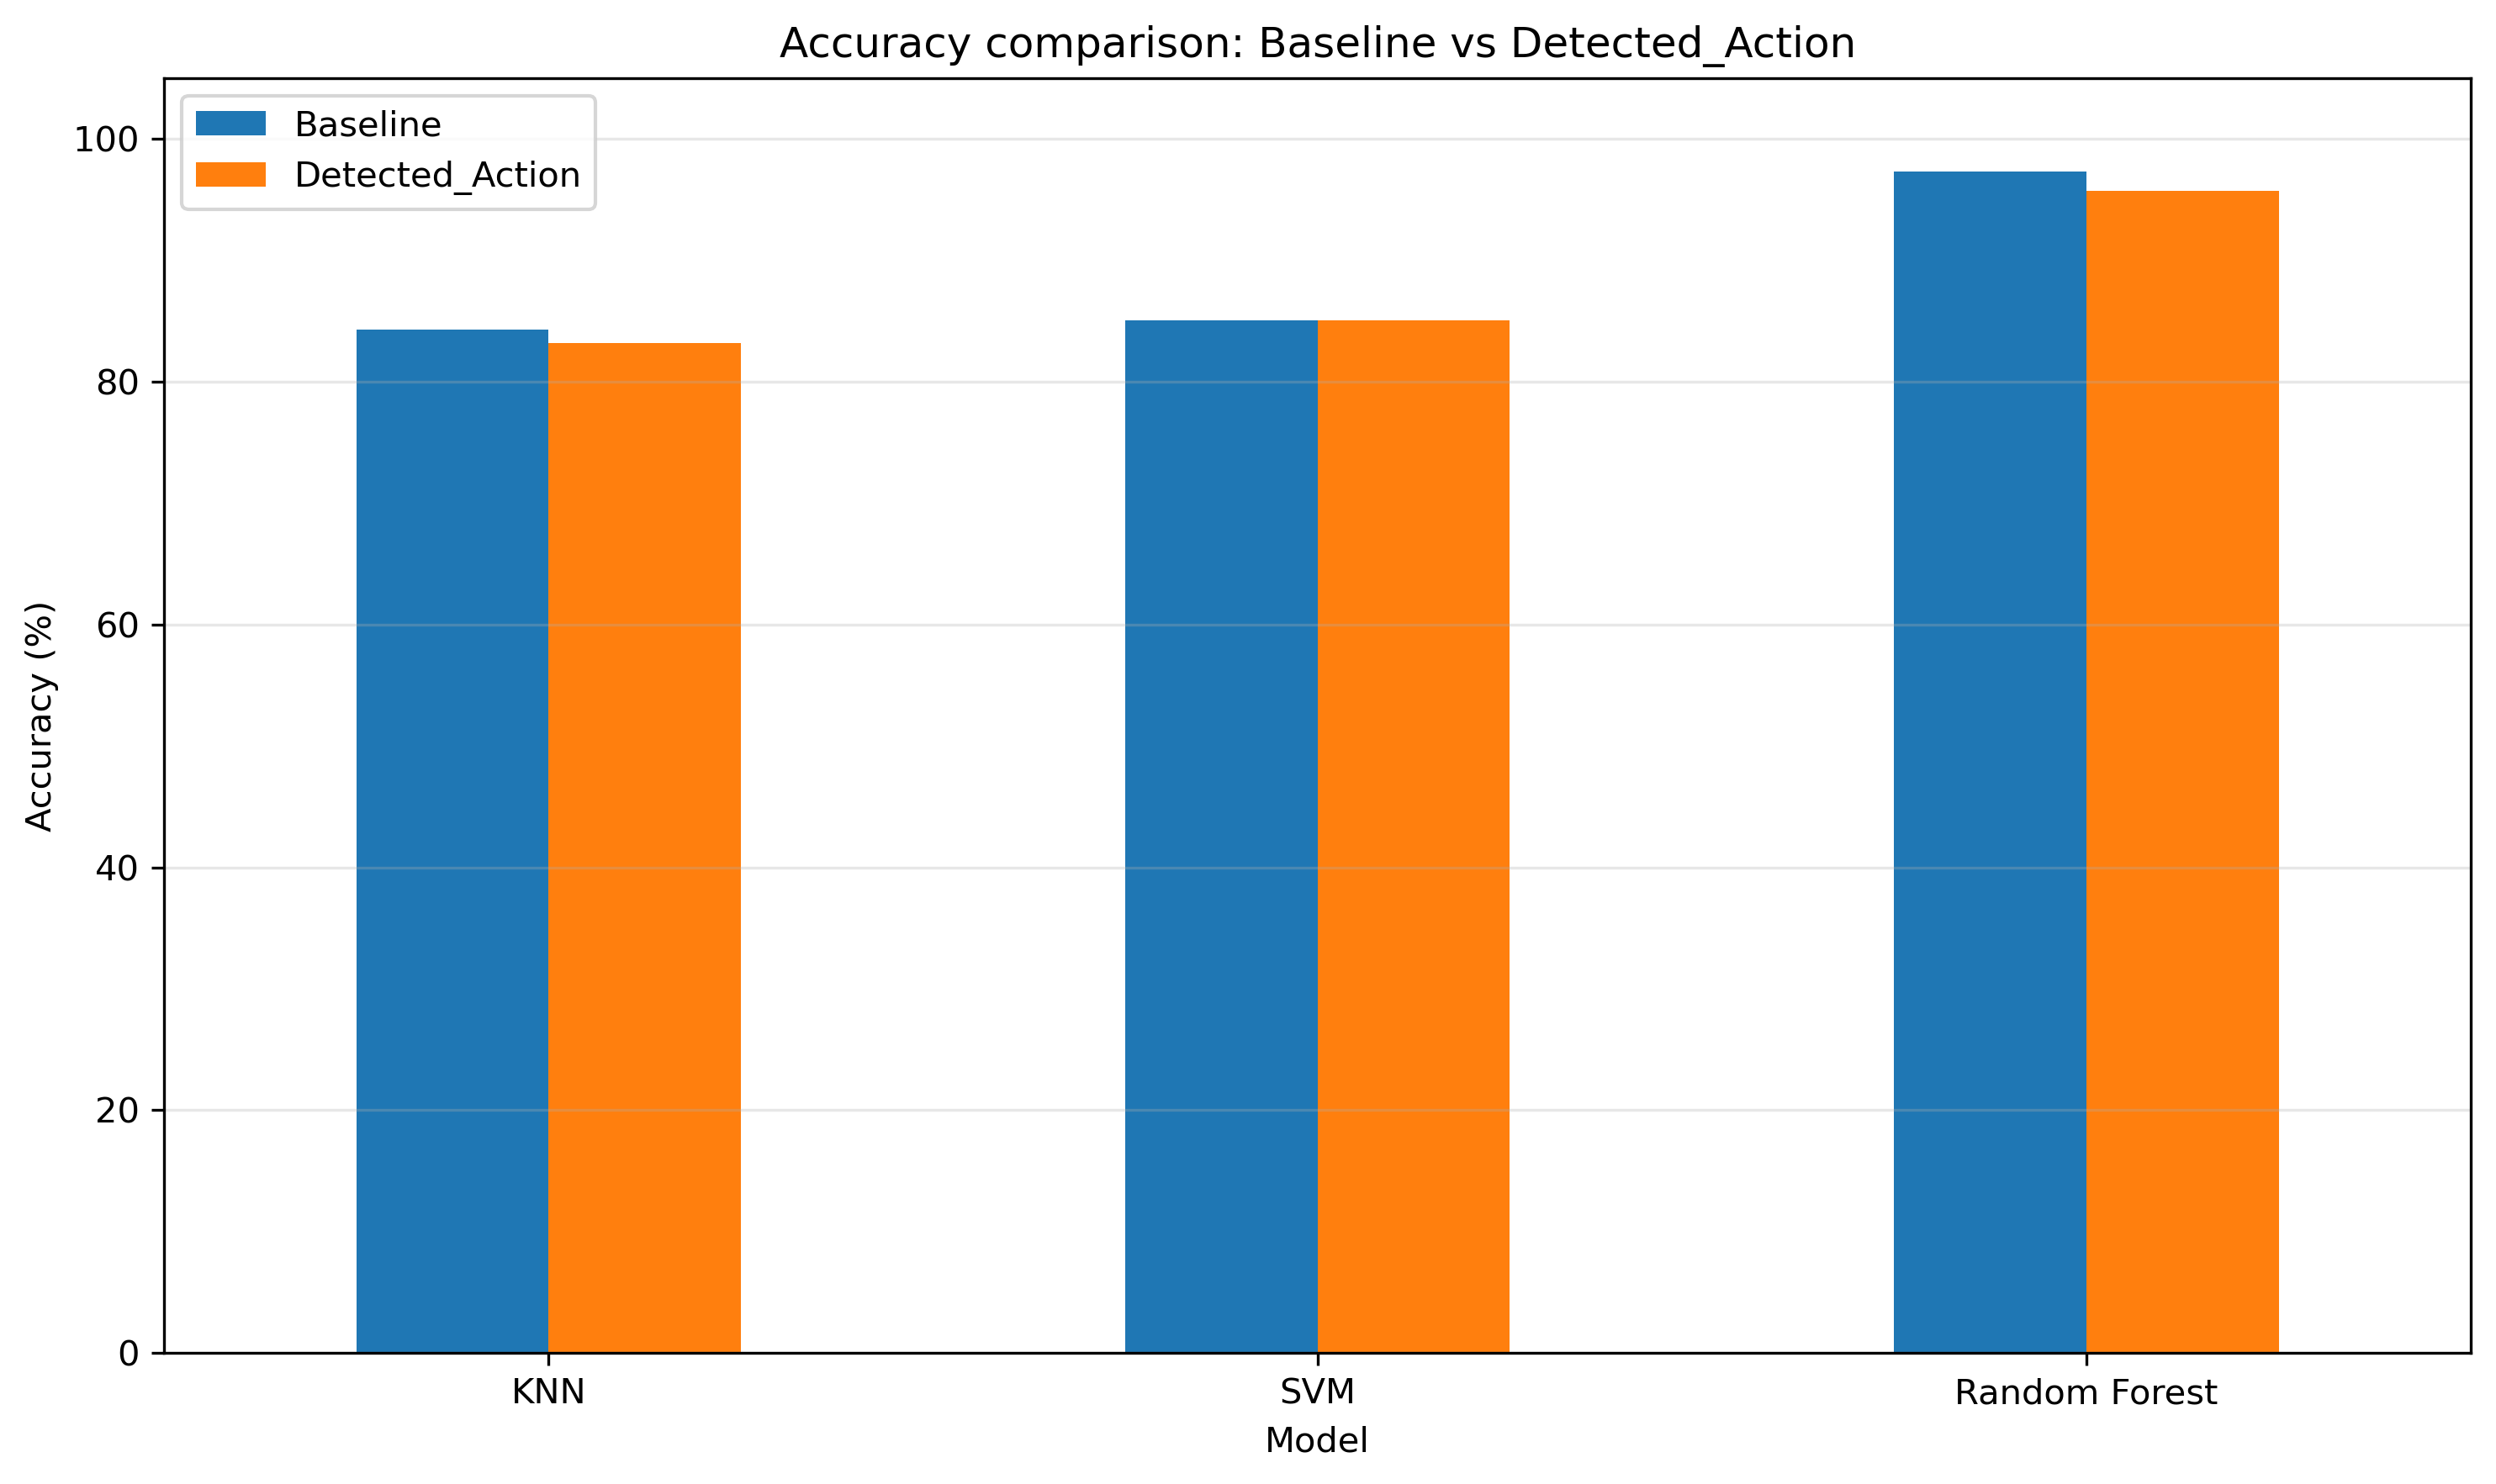
\includegraphics[width=0.7\linewidth]{../Results/Rise_Head/Comparisons/Accuracy_Baseline_vs_Detected_Action}
	\caption{بررسی اثر جداسازی فعالیت در برخاستن از صندلی}
	\label{fig:riseheadaccuracybaselinevsdetected}
\end{figure}
\paragraph{اهمیت ویژگی‌ها و انتخاب مؤلفه‌ها}

اثر تعداد مؤلفه‌های اصلی بر عملکرد مدل منتخب در
\autoref{fig:Rise_Head_all_metrics_vs_pca}
ارائه شده است. بر اساس این نمودار، با افزایش تعداد مؤلفه‌های اصلی، عملکرد مدل در ابتدا بهبود پیدا می‌کند؛ اما پس از حدود ۱۵ مؤلفه، افزودن مؤلفه‌های جدید لزوماً باعث افزایش قابل‌توجه معیارهای ارزیابی نمی‌شود. این موضوع نشان می‌دهد که بخش اصلی اطلاعات مورد نیاز برای تفکیک سطوح عملکردی در تعداد محدودتری از مؤلفه‌ها قرار دارد و استفاده از تمام مؤلفه‌ها برای آموزش مدل ضروری نیست.

\begin{figure}[H]
	\centering
	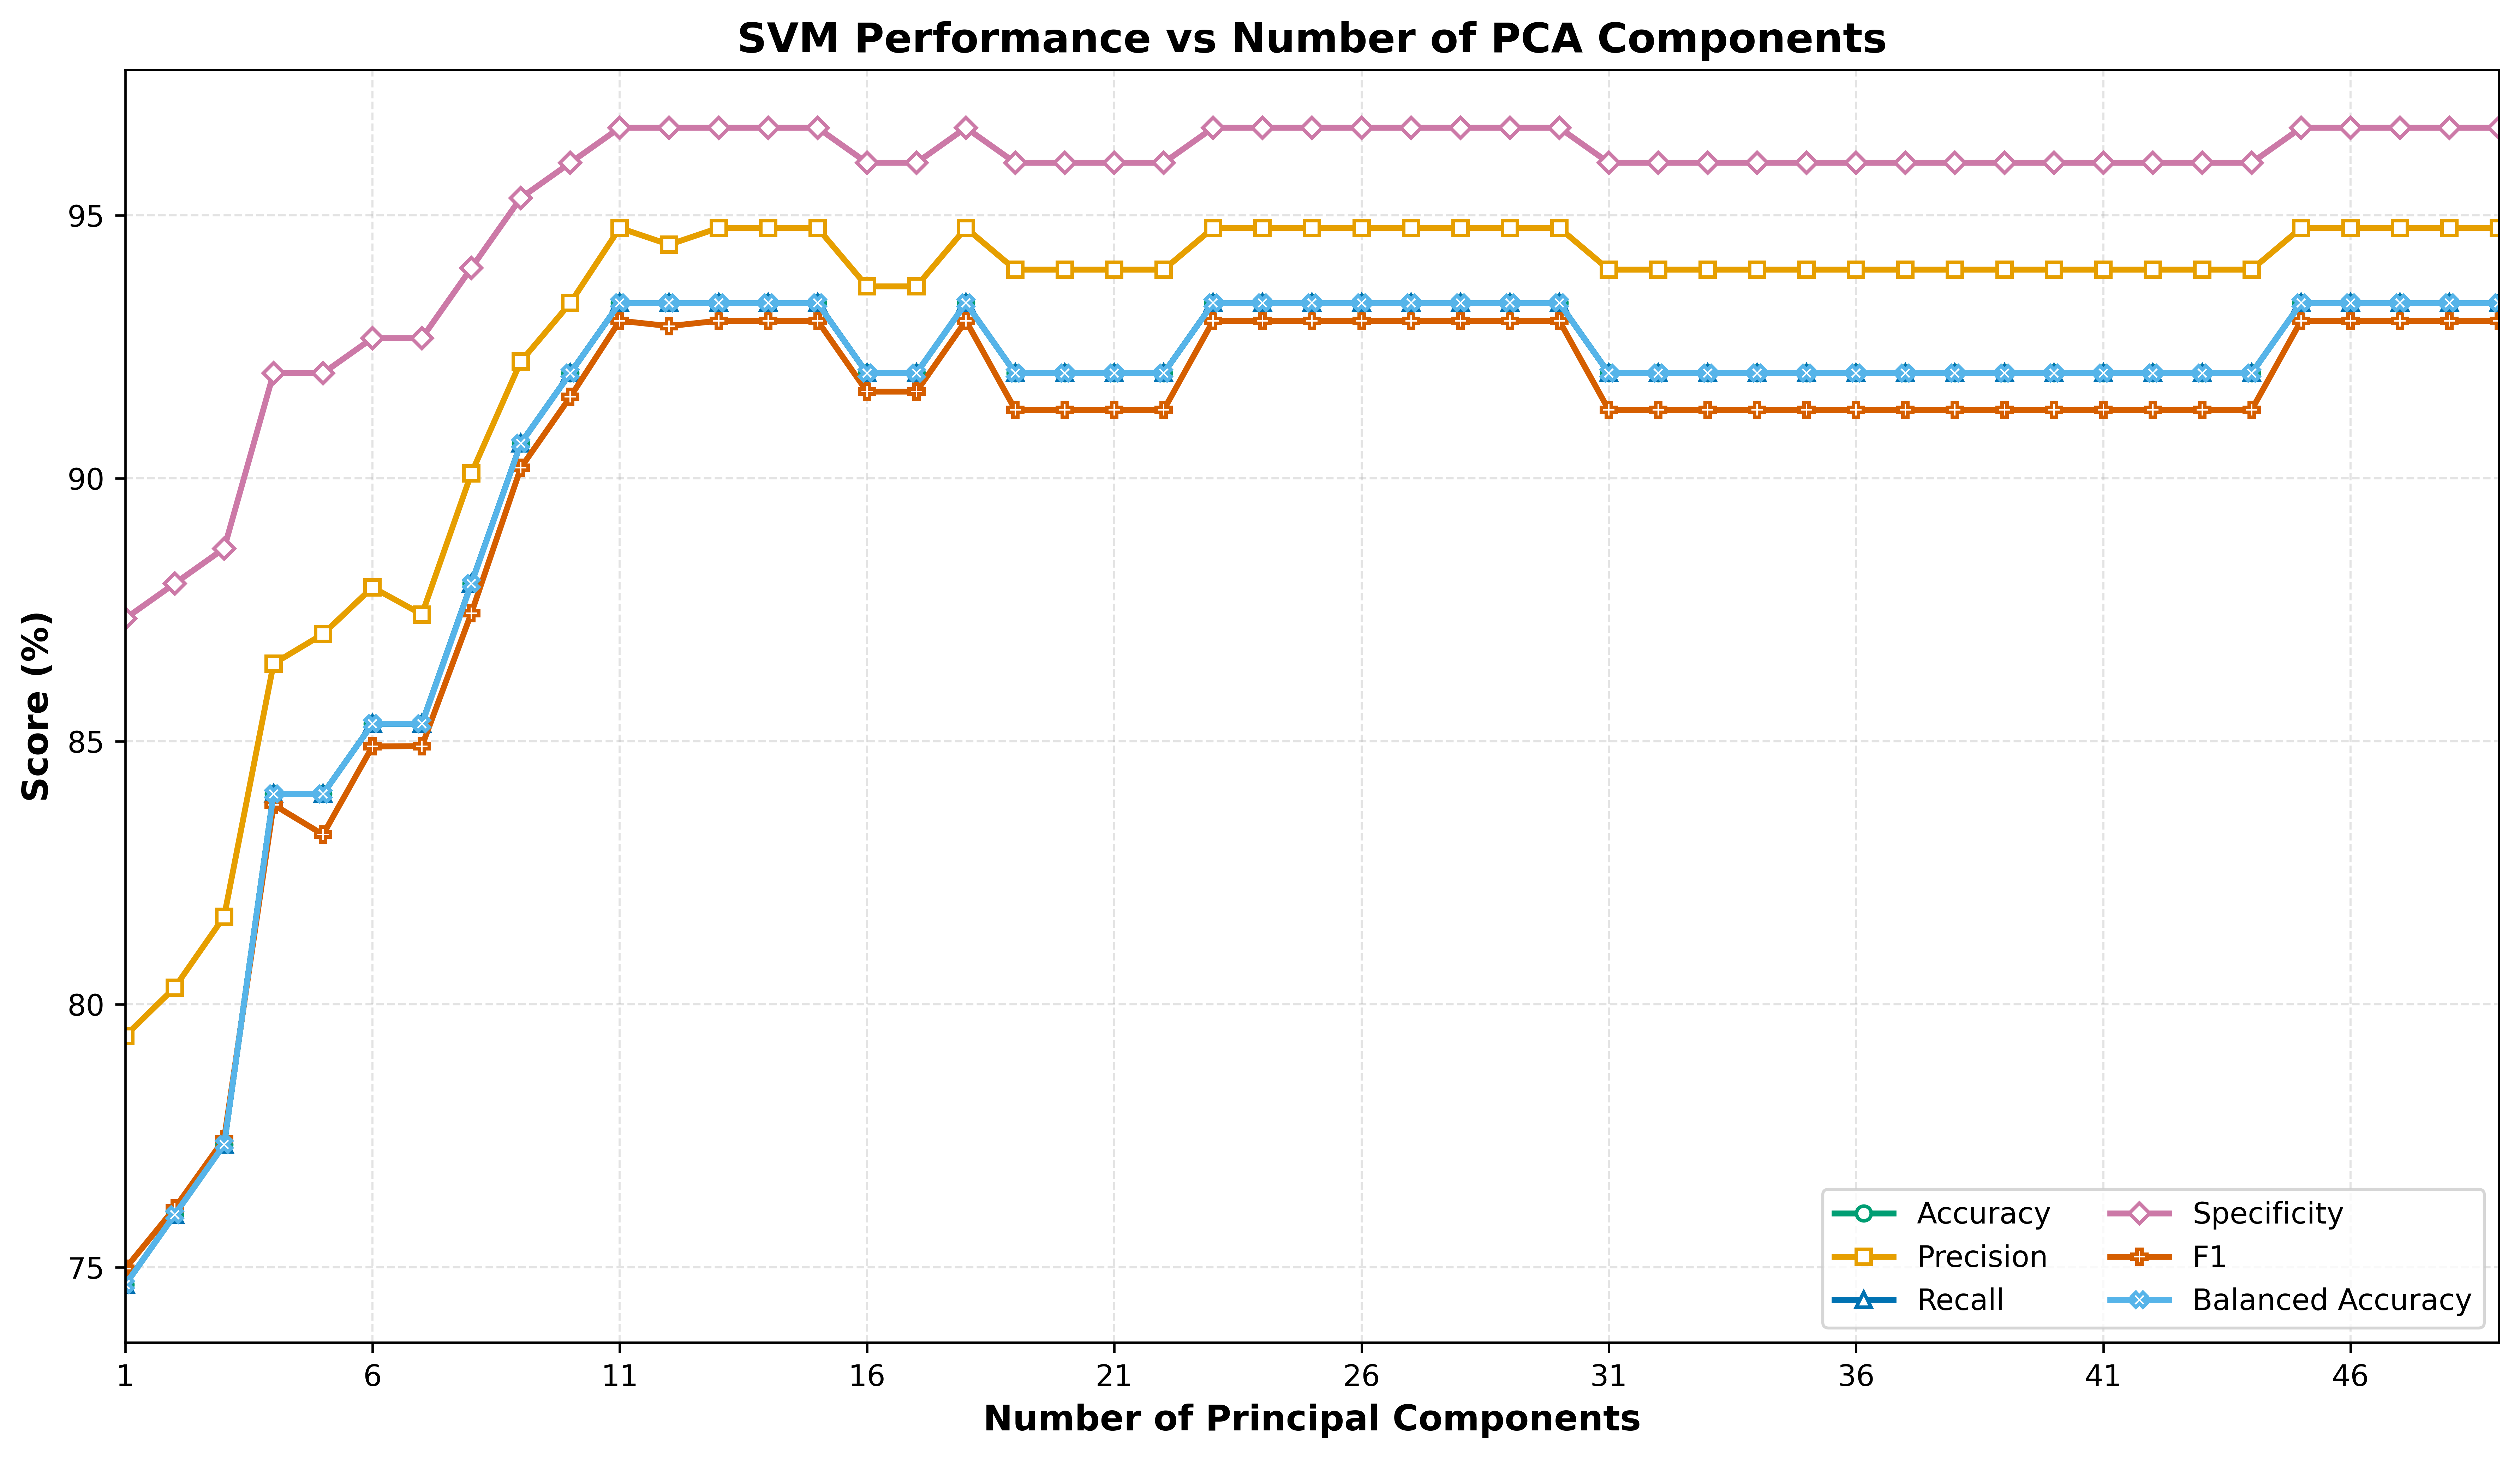
\includegraphics[width=0.7\linewidth]{../Results/Rise_Head/Normal/FindPrincipalComponents_PipelinePCA_Rise_Head/Figures/All_Metrics_vs_PCA}
	\caption{تغییر عملکرد مدل منتخب نسبت به تعداد مؤلفه‌های اصلی در فعالیت بالا آوردن سر}
	\label{fig:Rise_Head_all_metrics_vs_pca}
\end{figure}

در نهایت، بر اساس نمودار
\autoref{fig:Rise_Head_all_metrics_vs_pca}،
مدل‌ها در بازه ۵ تا ۱۵ مؤلفه اصلی دوباره مقایسه شدند تا مدل برتر و تعداد مؤلفه‌های اصلی بهینه تعیین شود. بر اساس نتایج به‌دست‌آمده در
\autoref{fig:Rise_Head_models_vs_pca_components}
، برای فعالیت بالا آوردن سر، مدل ماشین بردار پشتیبان با ۱۴ مؤلفه اصلی انتخاب شد. این ترکیب، ضمن کاهش قابل‌توجه تعداد ابعاد ورودی، دقتی بالاتر از حد نصاب ۹۰ درصد فراهم کرد. بنابراین، افزایش تعداد مؤلفه‌ها بیش از این مقدار، با توجه به افزایش پیچیدگی مدل، بهبود کافی و متناسبی در عملکرد ایجاد نمی‌کرد.

\begin{figure}[H]
	\centering
	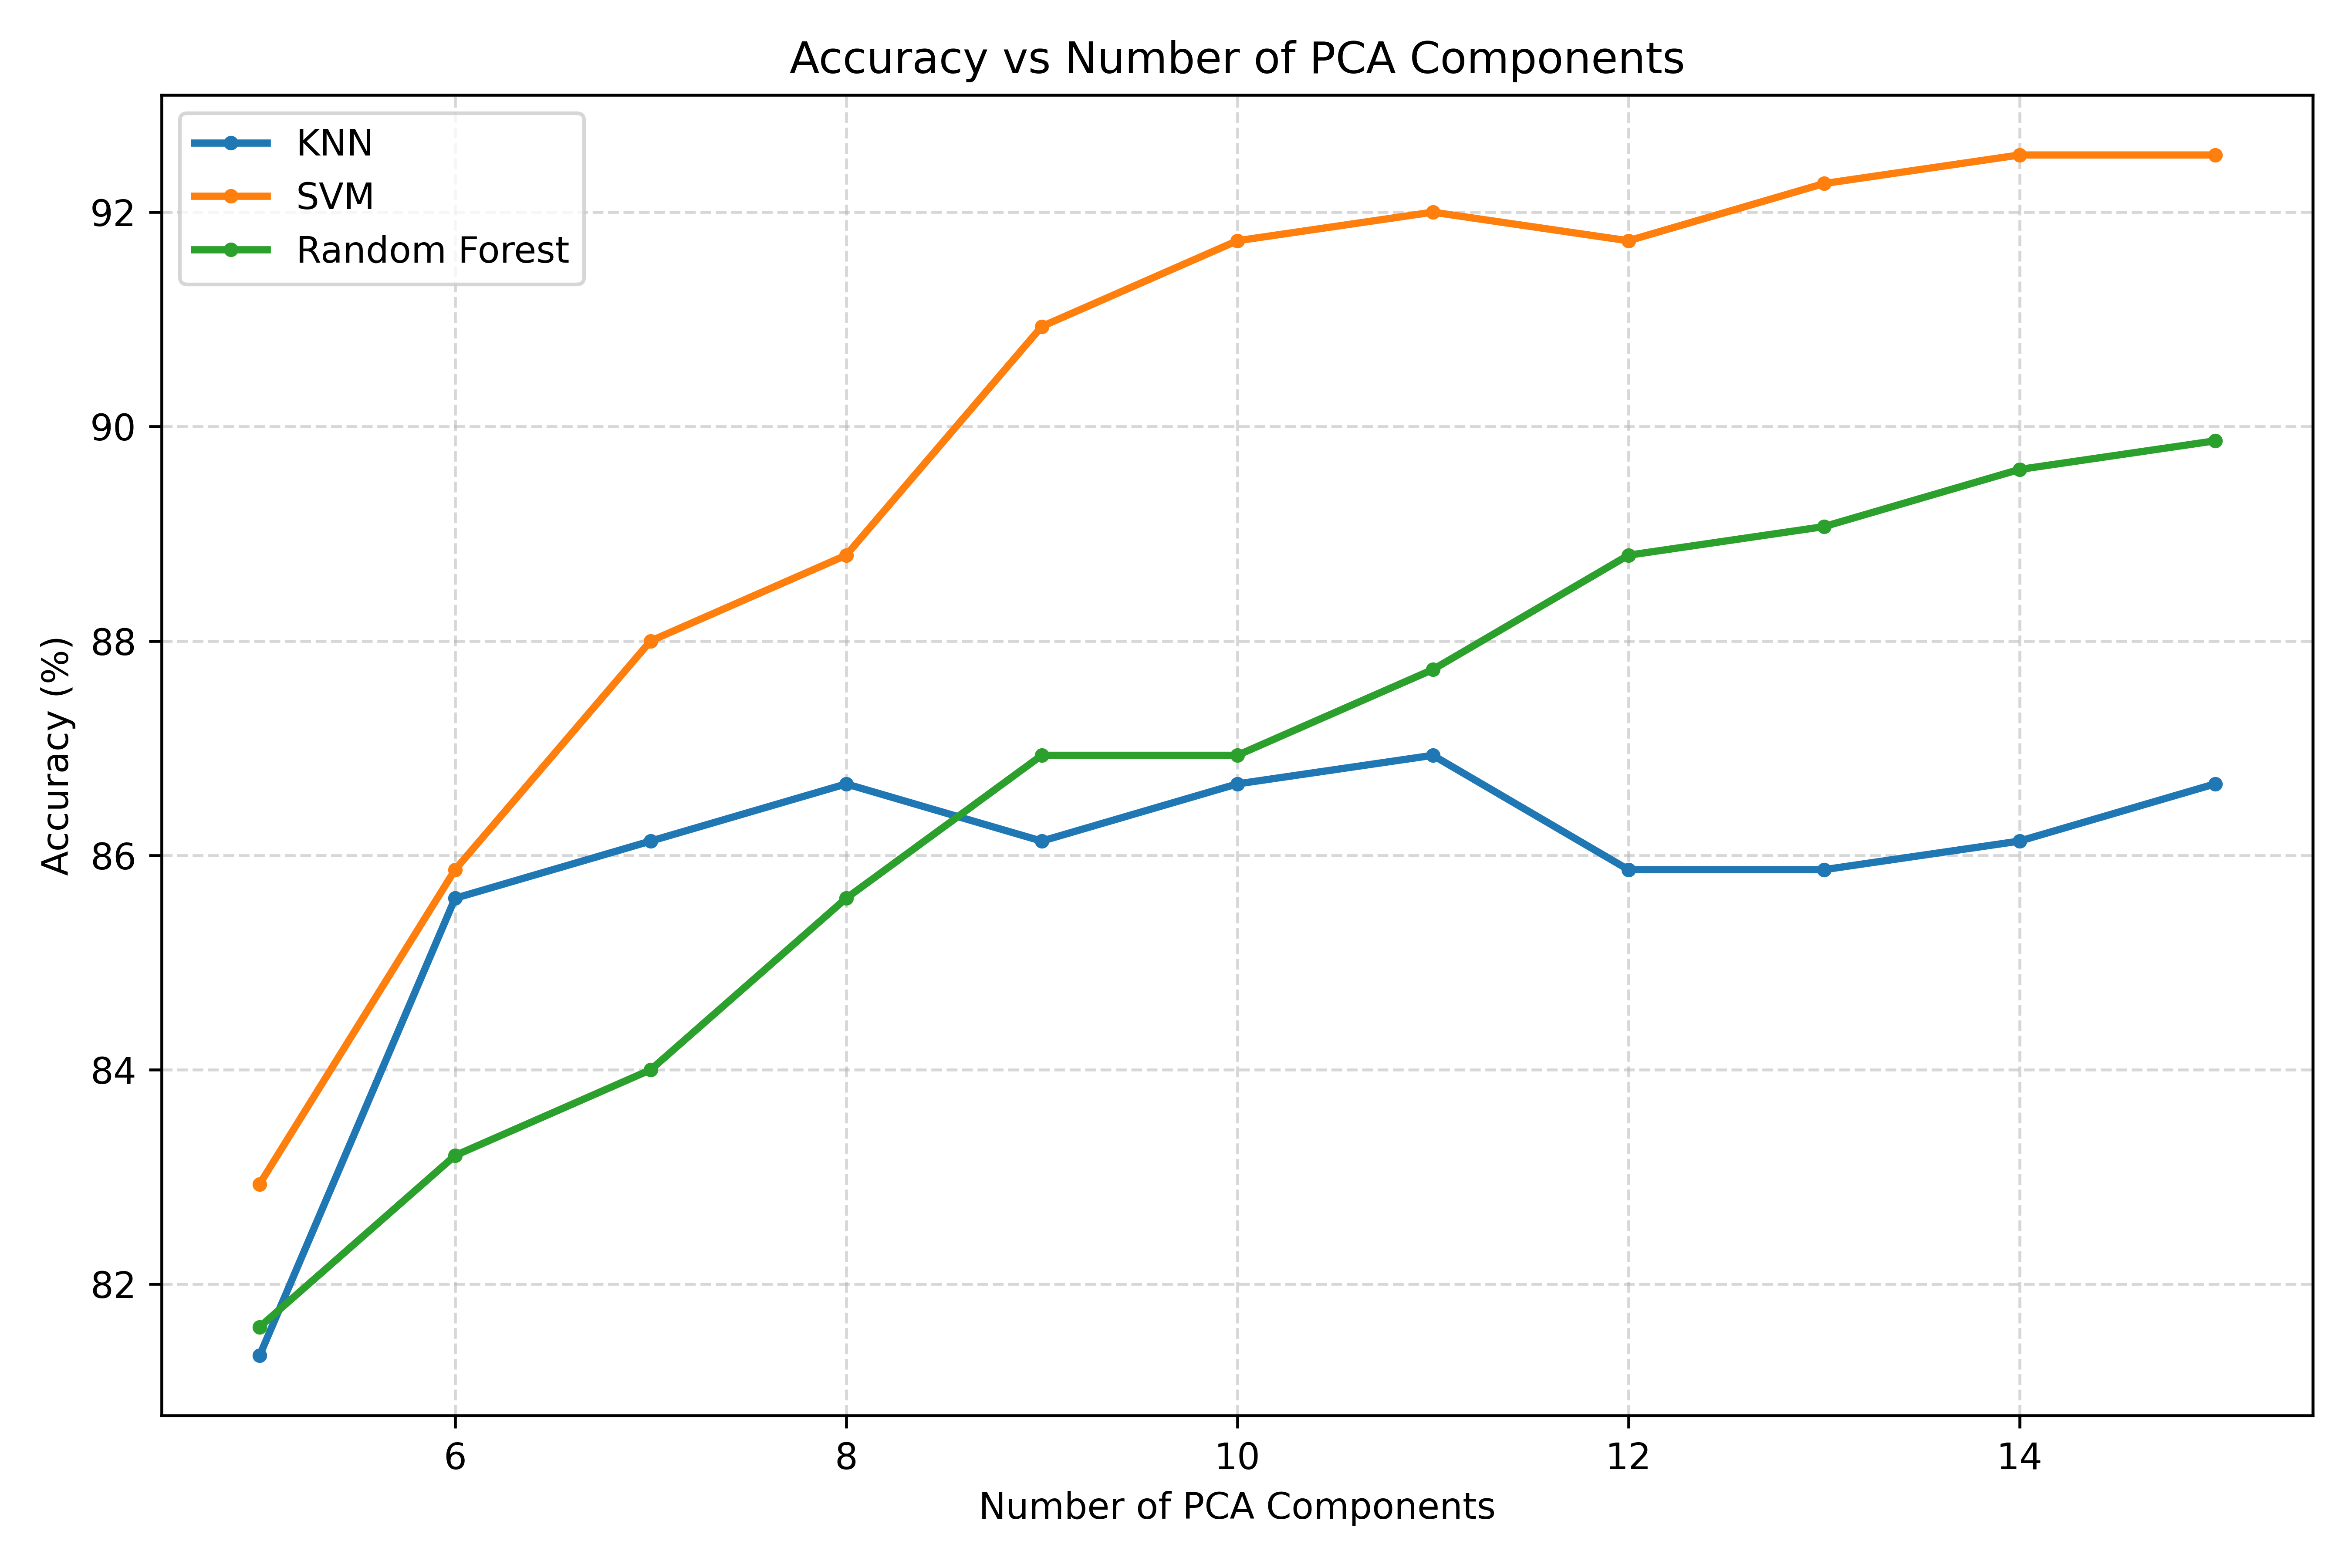
\includegraphics[width=0.7\linewidth]{../Results/Rise_Head/Normal/CompareNumberOfPrincipalComponents_PipelinePCA_Rise_Head/Figures/Accuracy_vs_PCA_Components}
	\caption{تغییر دقت مدل‌ها نسبت به تعداد مؤلفه‌های اصلی در فعالیت بالا آوردن سر}
	\label{fig:Rise_Head_models_vs_pca_components}
\end{figure}

\begin{table}[H]
	\centering
	\caption{تنظیمات منتخب فعالیت بالا آوردن سر برای مدل نهایی}
	\label{tab:Rise_Head_selected_setup}
	\begin{tabular}{lcccc}
		\toprule
		نوع داده & مدل منتخب & تعداد مؤلفه اصلی & معیار ارزیابی & حد نصاب معیار \\
		\midrule
		بدون جداسازی فعالیت & ماشین بردار پشتیبان & ۱۴ & دقت & ۹۰ درصد \\
		\bottomrule
	\end{tabular}
\end{table}

\paragraph{جمع‌بندی فعالیت بالا آوردن سر}

در فعالیت بالا آوردن سر، مدل منتخب معرفی‌شده در
\autoref{tab:Rise_Head_selected_setup}
با استفاده از اعتبارسنجی متقاطع طبقه‌بندی‌شده مورد ارزیابی قرار گرفت. نتایج نشان می‌دهند که ویژگی‌های حرکتی استخراج‌شده از حسگرها، به‌ویژه حسگر نصب‌شده روی پیشانی، قابلیت استفاده برای تفکیک سه سطح عملکردی شبیه‌سازی‌شده این فعالیت را دارند.

مدل ماشین بردار پشتیبان با استفاده از ۱۴ مؤلفه اصلی به‌عنوان مدل نهایی انتخاب شد. مؤلفه‌های اصلی منتخب در مجموع حدود ۷۰ درصد از واریانس داده‌های اولیه را در بر می‌گیرند. این نتیجه نشان می‌دهد که برای دستیابی به عملکرد مناسب مدل، حفظ تمام واریانس داده‌ها ضروری نبوده و بخش مؤثری از اطلاعات حرکتی در تعداد محدودی از مؤلفه‌ها خلاصه شده است.

در این ارزیابی، داده‌ها در هر مرحله به ۵ بخش تقسیم شدند و فرایند اعتبارسنجی ۵ مرتبه تکرار شد. نتایج حاصل از تقسیم‌بندی‌های مختلف در
\autoref{fig:Rise_Head_cv_fold_metrics}
ارائه شده‌اند. بررسی نتایج تقسیم‌بندی‌های مختلف امکان ارزیابی میزان ثبات مدل و وابستگی عملکرد آن به نحوه انتخاب داده‌های آموزش و آزمون را فراهم می‌کند.

\begin{figure}[H]
	\centering
	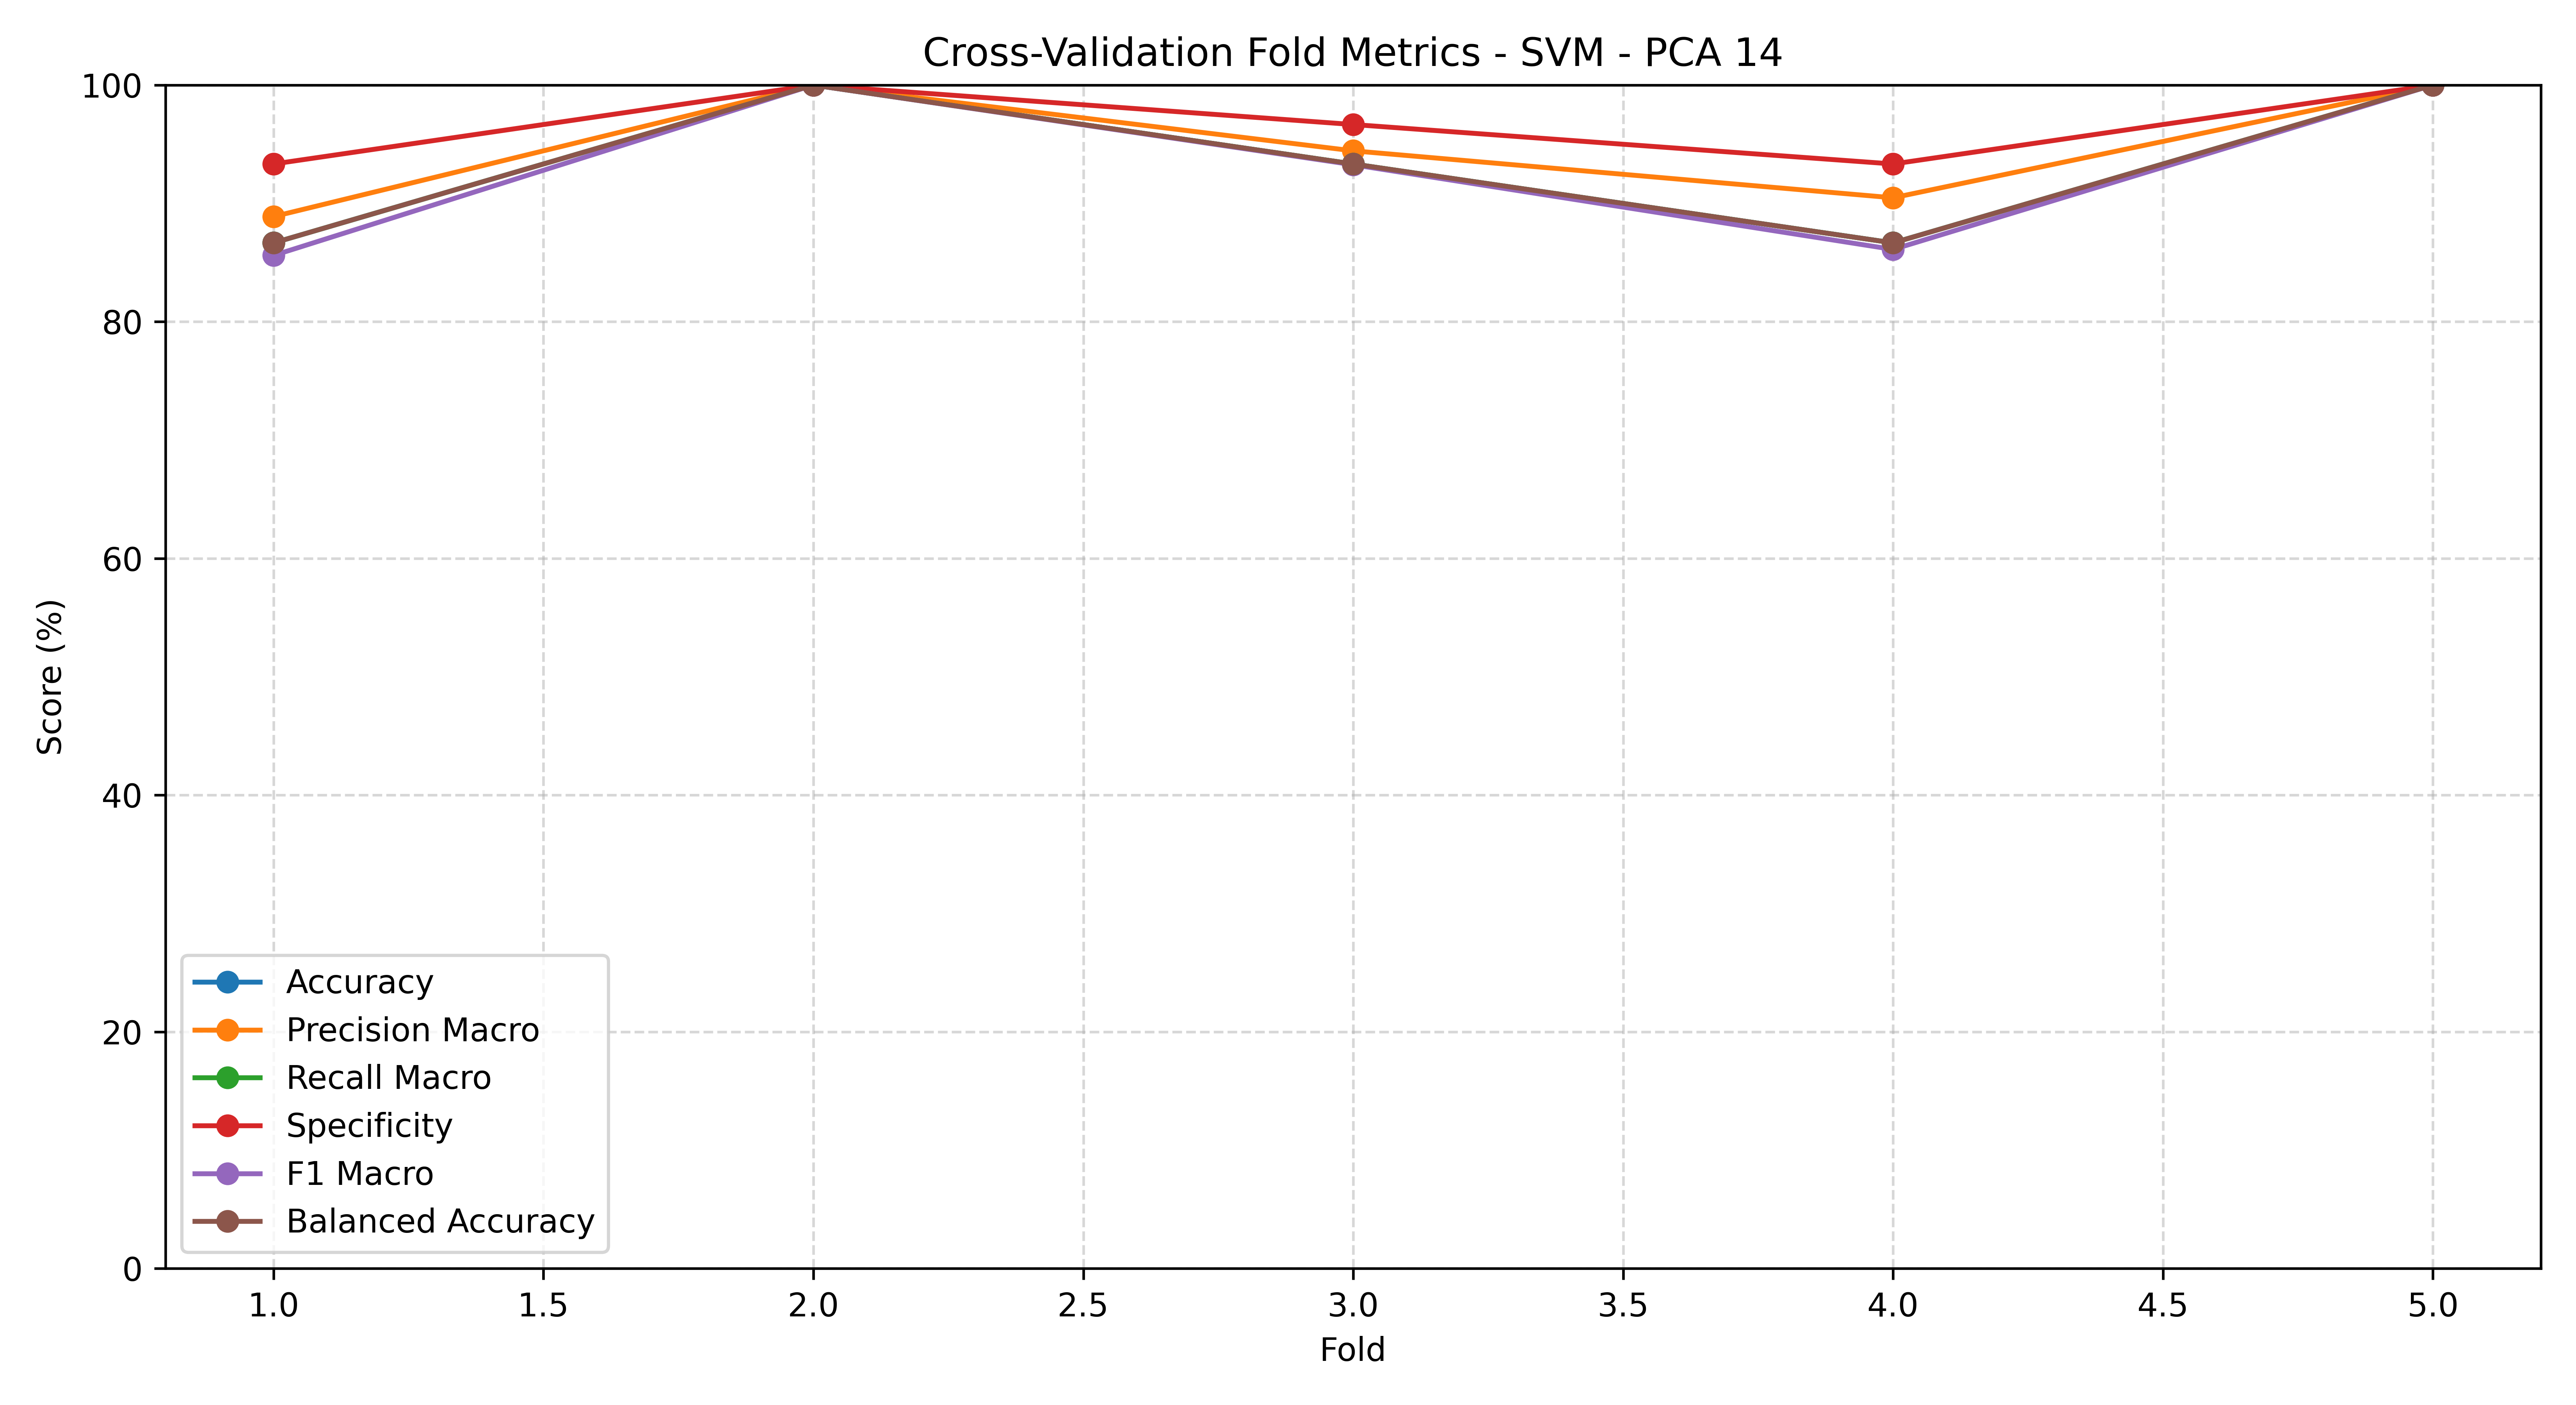
\includegraphics[width=0.7\linewidth]{../Results/Rise_Head/Final/Final_Model_SVM_PCA14/Figures/CV_Fold_Metrics}
	\caption{نتایج ارزیابی مدل منتخب برای فعالیت بالا آوردن سر در تقسیم‌بندی‌های مختلف}
	\label{fig:Rise_Head_cv_fold_metrics}
\end{figure}

در مجموع، نتایج این فعالیت نشان می‌دهند که تحلیل اطلاعات ثبت‌شده توسط حسگر پیشانی می‌تواند تغییرات مربوط به دامنه حرکت، سرعت اجرا و کنترل وضعیت سر را آشکار کند. اطلاعات حسگرهای نصب‌شده روی دست‌ها و پاها نیز می‌توانند برای شناسایی حرکات جبرانی احتمالی مورد استفاده قرار گیرند. بنابراین، تحلیل هم‌زمان داده‌های حسگرها امکان تفکیک الگوهای مختلف اجرای فعالیت بالا آوردن سر و شناسایی سطوح عملکردی شبیه‌سازی‌شده را فراهم کرده است.

